\documentclass[journal,12pt,twocolumn]{IEEEtran}

 \usepackage{setspace}
 \usepackage{gensymb}
 \usepackage{graphicx}

 \singlespacing

\graphicspath{ {/user/adarshsrivastava/desktop/Matrix Theory/Assignemnt_5} }
 \usepackage[cmex10]{amsmath}

 \usepackage{amsthm}
 \usepackage{mathrsfs}
 \usepackage{txfonts}
 \usepackage{stfloats}
 \usepackage{bm}
 \usepackage{cite}
 \usepackage{cases}
 \usepackage{subfig}

 \usepackage{longtable}
 \usepackage{multirow}

 \usepackage{enumitem}
 \usepackage{mathtools}
 \usepackage{steinmetz}
 \usepackage{tikz}
 \usepackage{circuitikz}
 \usepackage{verbatim}
 \usepackage{tfrupee}
 \usepackage[breaklinks=true]{hyperref}
 \usepackage{tkz-euclide}

 \usetikzlibrary{calc,math}
 \usepackage{listings}
     \usepackage{color}                                            %%
     \usepackage{array}                                            %%
     \usepackage{longtable}                                        %%
     \usepackage{calc}                                             %%
     \usepackage{multirow}                                         %%
     \usepackage{hhline}                                           %%
     \usepackage{ifthen}                                           %%
     \usepackage{lscape}     
 \usepackage{multicol}
 \usepackage{chngcntr}

 \DeclareMathOperator*{\Res}{Res}

 \renewcommand\thesection{\arabic{section}}
 \renewcommand\thesubsection{\thesection.\arabic{subsection}}
 \renewcommand\thesubsubsection{\thesubsection.\arabic{subsubsection}}

 \renewcommand\thesectiondis{\arabic{section}}
 \renewcommand\thesubsectiondis{\thesectiondis.\arabic{subsection}}
 \renewcommand\thesubsubsectiondis{\thesubsectiondis.\arabic{subsubsection}}


 \hyphenation{op-tical net-works semi-conduc-tor}
 \def\inputGnumericTable{}                                 %%

 \lstset{
 %language=C,
 frame=single, 
 breaklines=true,
 columns=fullflexible
 }
\begin{document}


 \newtheorem{theorem}{Theorem}[section]
 \newtheorem{problem}{Problem}
 \newtheorem{proposition}{Proposition}[section]
 \newtheorem{lemma}{Lemma}[section]
 \newtheorem{corollary}[theorem]{Corollary}
 \newtheorem{example}{Example}[section]
 \newtheorem{definition}[problem]{Definition}

 \newcommand{\BEQA}{\begin{eqnarray}}
 \newcommand{\EEQA}{\end{eqnarray}}
 \newcommand{\define}{\stackrel{\triangle}{=}}
 \bibliographystyle{IEEEtran}
 \providecommand{\mbf}{\mathbf}
 \providecommand{\pr}[1]{\ensuremath{\Pr\left(#1\right)}}
 \providecommand{\qfunc}[1]{\ensuremath{Q\left(#1\right)}}
 \providecommand{\sbrak}[1]{\ensuremath{{}\left[#1\right]}}
 \providecommand{\lsbrak}[1]{\ensuremath{{}\left[#1\right.}}
 \providecommand{\rsbrak}[1]{\ensuremath{{}\left.#1\right]}}
 \providecommand{\brak}[1]{\ensuremath{\left(#1\right)}}
 \providecommand{\lbrak}[1]{\ensuremath{\left(#1\right.}}
 \providecommand{\rbrak}[1]{\ensuremath{\left.#1\right)}}
 \providecommand{\cbrak}[1]{\ensuremath{\left\{#1\right\}}}
 \providecommand{\lcbrak}[1]{\ensuremath{\left\{#1\right.}}
 \providecommand{\rcbrak}[1]{\ensuremath{\left.#1\right\}}}
 \theoremstyle{remark}
 \newtheorem{rem}{Remark}
 \newcommand{\sgn}{\mathop{\mathrm{sgn}}}
 \providecommand{\abs}[1]{\left\vert#1\right\vert}
 \providecommand{\res}[1]{\Res\displaylimits_{#1}} 
 \providecommand{\norm}[1]{\left\lVert#1\right\rVert}
 %\providecommand{\norm}[1]{\lVert#1\rVert}
 \providecommand{\mtx}[1]{\mathbf{#1}}
 \providecommand{\mean}[1]{E\left[ #1 \right]}
 \providecommand{\fourier}{\overset{\mathcal{F}}{ \rightleftharpoons}}
 %\providecommand{\hilbert}{\overset{\mathcal{H}}{ \rightleftharpoons}}
 \providecommand{\system}{\overset{\mathcal{H}}{ \longleftrightarrow}}
 	%\newcommand{\solution}[2]{\textbf{Solution:}{#1}}
 \newcommand{\solution}{\noindent \textbf{Solution: }}
 \newcommand{\cosec}{\,\text{cosec}\,}
 \providecommand{\dec}[2]{\ensuremath{\overset{#1}{\underset{#2}{\gtrless}}}}
 \newcommand{\myvec}[1]{\ensuremath{\begin{pmatrix}#1\end{pmatrix}}}
 \newcommand{\mydet}[1]{\ensuremath{\begin{vmatrix}#1\end{vmatrix}}}
 \numberwithin{equation}{subsection}
 \makeatletter
 \@addtoreset{figure}{problem}
 \makeatother
 \let\StandardTheFigure\thefigure
 \let\vec\mathbf
 \renewcommand{\thefigure}{\theproblem}
 \def\putbox#1#2#3{\makebox[0in][l]{\makebox[#1][l]{}\raisebox{\baselineskip}[0in][0in]{\raisebox{#2}[0in][0in]{#3}}}}
      \def\rightbox#1{\makebox[0in][r]{#1}}
      \def\centbox#1{\makebox[0in]{#1}}
      \def\topbox#1{\raisebox{-\baselineskip}[0in][0in]{#1}}
      \def\midbox#1{\raisebox{-0.5\baselineskip}[0in][0in]{#1}}
 \vspace{3cm}
 \title{Assignment 2}
 \author{Matish Singh Tanwar}
 \maketitle
 \newpage
 \bigskip
 %\renewcommand{\thefigure}{\theenumi}
 \renewcommand{\thetable}{\theenumi}
\vspace{1.0cm}
\begin{abstract}
This document finds the equation of a plane which is at a distance of 7 units from origin and normal to $\myvec{3\\5\\6}$
\end{abstract}
\vspace{0.5cm}
Download all python codes from 
\begin{lstlisting}
https://github.com/Matish007/Matrix-Theory-EE5609-/tree/master/Assignment_2/codes
\end{lstlisting}
%
and latex-tikz codes from 
\begin{lstlisting}
https://github.com/Matish007/Matrix-Theory-EE5609-/tree/master/Assignment_2
\end{lstlisting}
%
\vspace{0.5mm}
\section{Problem}
Find the equation of a plane which is at a distance of 7 units from origin and normal to $\myvec{3\\5\\6}$\\
\begin{align}\label{1}
    \vec{n}=\myvec{3\\5\\6}
\end{align}
\section{Explanation}
Let the equation of plane be:-\\
\begin{align}\label{2}
   \vec{n}^T\vec{x} = c
\end{align}
where $\vec{n}$=normal vector to the plane\\
The distance from the origin is given by:-
\begin{align}
    \frac{\abs{c}}{\norm{\vec{n}}} = 7\label{3}\\
    \norm{\vec{n}}=\sqrt{3^2+5^2+6^2}=\sqrt{70}\label{4}
\end{align}
Substituting equation \eqref{4} in \eqref{3} we get,
\begin{align}
    \frac{\abs{c}}{\sqrt{70}}=7\label{5}\\
    c=\pm{7\sqrt{70}}\label{6}
\end{align}
Substituting equation \eqref{1},\eqref{6} in \eqref{2} we get two equation of planes,
\begin{align}
    \boxed{\myvec{3 & 5 & 6}\vec{x}=7\sqrt{70}}\label{7}\\
     \boxed{\myvec{3 & 5 & 6}\vec{x}=-7\sqrt{70}}\label{8}
\end{align}
Equation \eqref{7} and \eqref{8} gives us the equation of two planes which are at a distance of 7 units from origin and normal to $\myvec{3\\5\\6}$
\begin{figure}[h!]
	\centering
	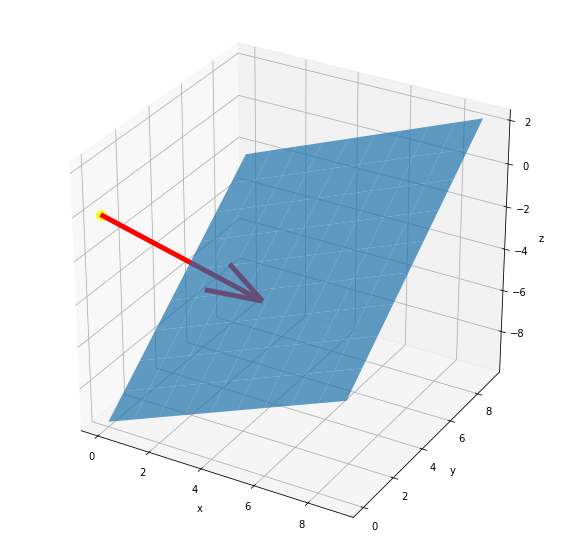
\includegraphics[width=\columnwidth]{plane.png}
	\caption{Planes with Normal vectors}
	\label{myfig}
\end{figure}
\end{document}